\section{Usage}
\subsection{Schematics}

\begin{frame}[fragile]
\frametitle{Sample Process Hierarchy}
\begin{alltt}\footnotesize
init(1)-+-dnsmasq(2162)
        |-klogd(2175)
        |-lxc-start(2964)---init(2966)----+-init(2972)
        |                                 |-sh(2971)
        |                                 `-syslogd(2969)
        |
        |
        |-lxc-start(2974)---init(2976)----+-init(2982)
        |                                 |-sh(2981)
        |                                 `-syslogd(2979)
        |
        |
        |-netserver(2167)
        |-sh(2179)
        |-syslogd(2173)
        `-udevd(962)-+-udevd(1189)
                     `-udevd(1190)
\end{alltt}\normalsize
\end{frame}

\begin{frame}[fragile]
\frametitle{Process IDs}
\begin{alltt}\footnotesize
init(1)-+-dnsmasq(2162)
        |-klogd(2175)
        |-lxc-start(2964)---init(2966)\colorwrevert{Green}{(1)}-+-init(2972)\colorwrevert{Green}{(7)}
        |                                 |-sh(2971)\colorwrevert{Green}{(6)}
        |                                 `-syslogd(2969)\colorwrevert{Green}{(4)}
        |
        |
        |-lxc-start(2974)---init(2976)\colorwrevert{Red}{(1)}-+-init(2982)\colorwrevert{Red}{(7)}
        |                                 |-sh(2981)\colorwrevert{Red}{(6)}
        |                                 `-syslogd(2979)\colorwrevert{Red}{(4)}
        |
        |
        |-netserver(2167)
        |-sh(2179)
        |-syslogd(2173)
        `-udevd(962)-+-udevd(1189)
                     `-udevd(1190)
\end{alltt}\normalsize
\end{frame}

\begin{frame}[fragile]
\frametitle{Namespace Segregation}
\begin{alltt}\footnotesize
init(1)-+-dnsmasq(2162)
        |-klogd(2175)
        |-lxc-start(2964)---\colorbox{LightGreen}{init(2966)\colorwrevert{Green}{(1)}-+-init(2972)\colorwrevert{Green}{(7)}    }
        |                   \colorbox{LightGreen}{              |-sh(2971)\colorwrevert{Green}{(6)}      }
        |                   \colorbox{LightGreen}{              `-syslogd(2969)\colorwrevert{Green}{(4)} }
        |                   \colorwrevert{Green}{PID Namespace 1}
        |
        |-lxc-start(2974)---\colorbox{LightRed}{init(2976)\colorwrevert{Red}{(1)}-+-init(2982)\colorwrevert{Red}{(7)}    }
        |                   \colorbox{LightRed}{              |-sh(2981)\colorwrevert{Red}{(6)}      }
        |                   \colorbox{LightRed}{              `-syslogd(2979)\colorwrevert{Red}{(4)} }
        |                   \colorwrevert{Red}{PID Namespace 2}
        |
        |-netserver(2167)
        |-sh(2179)
        |-syslogd(2173)
        `-udevd(962)-+-udevd(1189)
                     `-udevd(1190)
\end{alltt}\normalsize
\end{frame}

\begin{frame}[fragile]
\frametitle{Filesystem Segregation}
\framesubtitle{"chroot on steroids"}
\begin{alltt}\footnotesize
init(1)-+-dnsmasq(2162)
        |-klogd(2175)       \colorwrevert{Green}{root: /var/lib/lxc/foo1/rootfs/}
        |-lxc-start(2964)---\colorbox{LightGreen}{init(2966)\colorwrevert{Green}{(1)}-+-init(2972)\colorwrevert{Green}{(7)}    }
        |                   \colorbox{LightGreen}{              |-sh(2971)\colorwrevert{Green}{(6)}      }
        |                   \colorbox{LightGreen}{              `-syslogd(2969)\colorwrevert{Green}{(4)} }
        |                   \colorwrevert{Green}{PID Namespace 1}
        |                   \colorwrevert{Red}{root: /var/lib/lxc/foo2/rootfs/}
        |-lxc-start(2974)---\colorbox{LightRed}{init(2976)\colorwrevert{Red}{(1)}-+-init(2982)\colorwrevert{Red}{(7)}    }
        |                   \colorbox{LightRed}{              |-sh(2981)\colorwrevert{Red}{(6)}      }
        |                   \colorbox{LightRed}{              `-syslogd(2979)\colorwrevert{Red}{(4)} }
        |                   \colorwrevert{Red}{PID Namespace 2}
        |
        |-netserver(2167)
        |-sh(2179)
        |-syslogd(2173)
        `-udevd(962)-+-udevd(1189)
                     `-udevd(1190)
\end{alltt}\normalsize
\end{frame}

\begin{frame}[fragile]
\frametitle{CPU Partitioning}
\begin{alltt}\footnotesize
init(1)-+-dnsmasq(2162)
        |-klogd(2175)       \colorwrevert{Green}{root: /var/lib/lxc/foo1/rootfs/}
  ,-----|-lxc-start(2964)---\colorbox{LightGreen}{init(2966)\colorwrevert{Green}{(1)}-+-init(2972)\colorwrevert{Green}{(7)}    }
  |     |       \colorwrevert{Green}{25\%}         \colorbox{LightGreen}{              |-sh(2971)\colorwrevert{Green}{(6)}      }
  |     |                   \colorbox{LightGreen}{              `-syslogd(2969)\colorwrevert{Green}{(4)} }
  |     |                   \colorwrevert{Green}{PID Namespace 1}
  |     |                   \colorwrevert{Red}{root: /var/lib/lxc/foo2/rootfs/}
1 core  |-lxc-start(2974)---\colorbox{LightRed}{init(2976)\colorwrevert{Red}{(1)}-+-init(2982)\colorwrevert{Red}{(7)}    }
  |     |       \colorwrevert{Red}{75\%}         \colorbox{LightRed}{              |-sh(2981)\colorwrevert{Red}{(6)}      }
  |     |                   \colorbox{LightRed}{              `-syslogd(2979)\colorwrevert{Red}{(4)} }
  |     |                   \colorwrevert{Red}{PID Namespace 2}
  `-----|-----------------------------------------------------
        |-netserver(2167)
        |-sh(2179)
        |-syslogd(2173)
        `-udevd(962)-+-udevd(1189)
                     `-udevd(1190)
\end{alltt}\normalsize
\end{frame}

\subsection{Demo}

\begin{frame}{Demo}
\begin{enumerate}
\item Start 2 containers
\item Check PIDs
\item Assign them a single core on the host
\item Balance CPU usage 25\% - 75\%
\end{enumerate}
\end{frame}

\subsection{Benchmarks}

\begin{frame}{System Performance}
	\begin{columns}[T]
		\begin{column}{.5\textwidth}
			\begin{block}{\centering \textbf{CPU performance} \\ Linpack}
				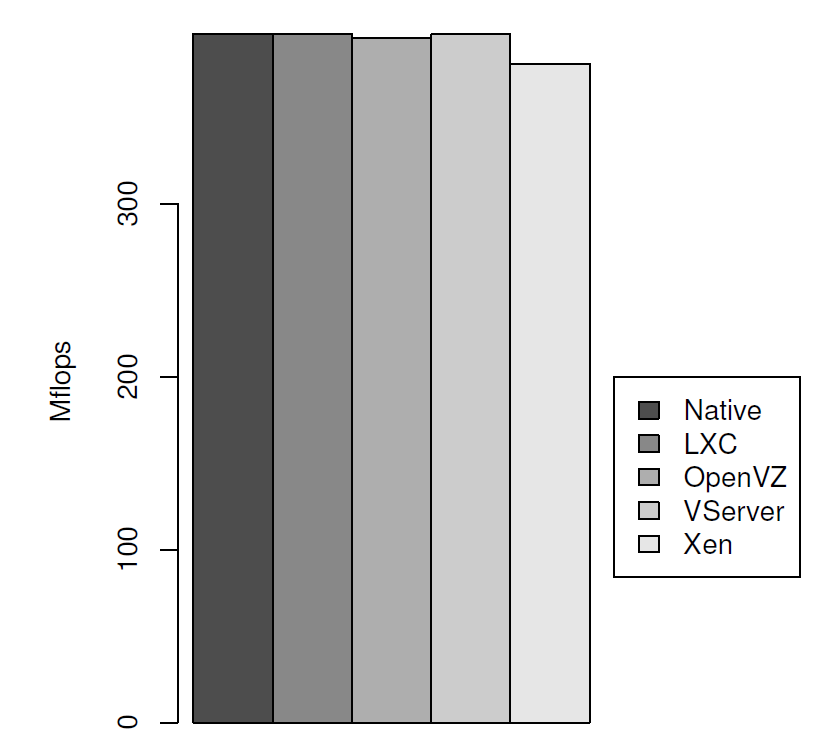
\includegraphics[width=\textwidth]{img/cpu_perf_linpack.png}
			\end{block}
		\end{column}
		\begin{column}{.5\textwidth}
			\begin{block}{\centering \textbf{Mem throughput} \\ Stream}
				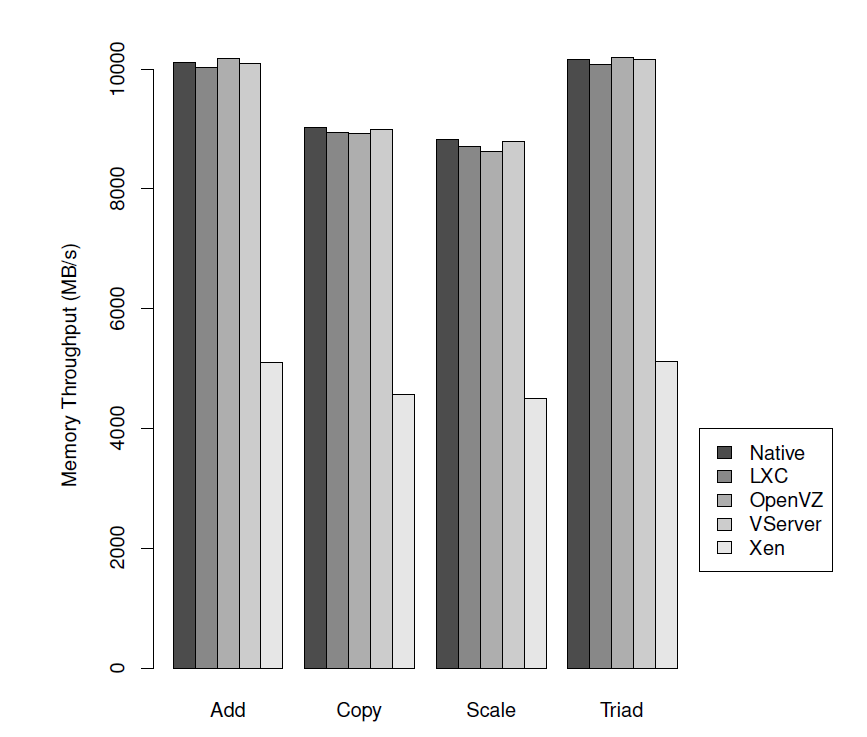
\includegraphics[width=\textwidth]{img/mem_throughput_stream.png}
			\end{block}
		\end{column}
	\end{columns}
\end{frame}

\begin{frame}{Networking Performance}
	\begin{columns}[T]
		\begin{column}{.5\textwidth}
			\begin{block}{\centering \textbf{Bandwidth} \\ NetPIPE}
				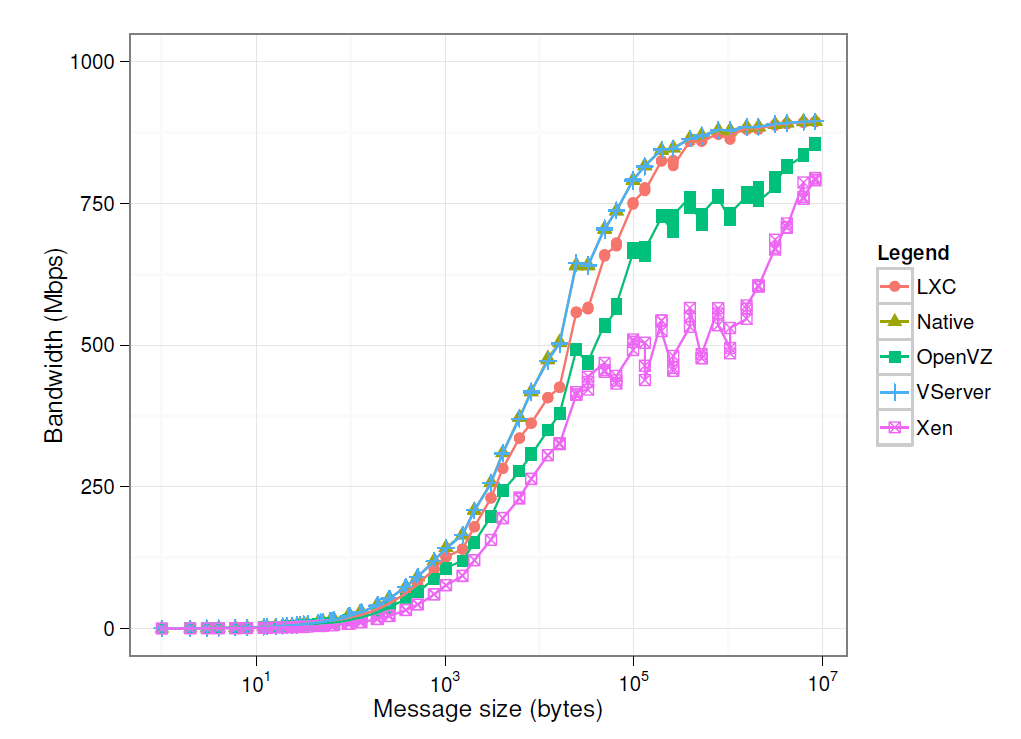
\includegraphics[width=\textwidth]{img/net_bandwidth_netpipe.png}
			\end{block}
		\end{column}
		\begin{column}{.5\textwidth}
			\begin{block}{\centering \textbf{Latency} \\ NetPIPE}
				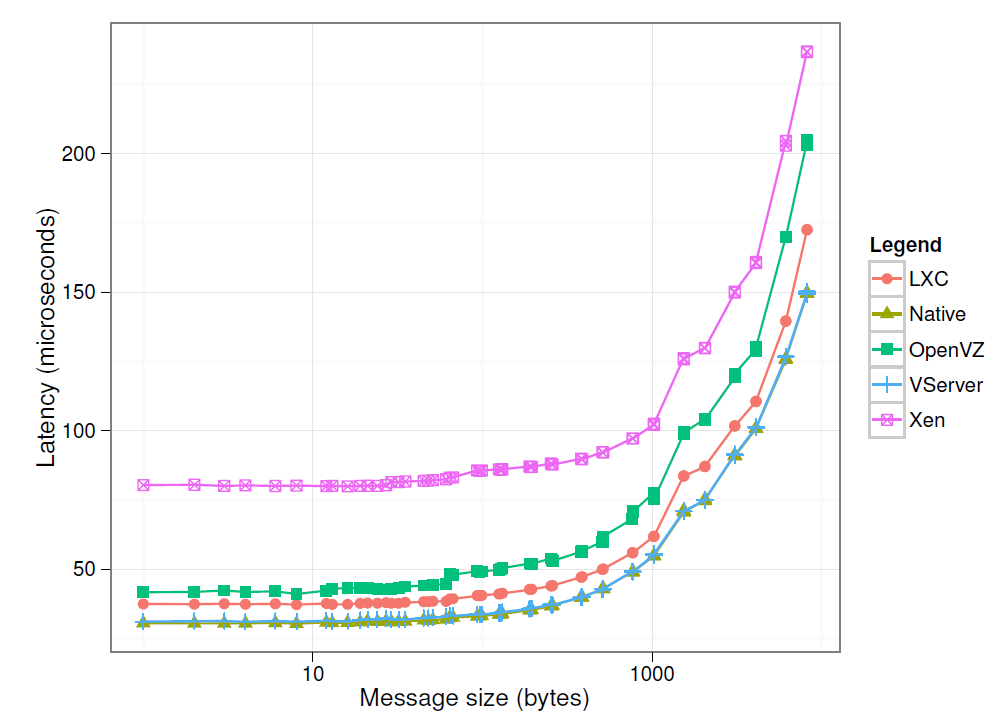
\includegraphics[width=\textwidth]{img/net_latency_netpipe.png}
			\end{block}
		\end{column}
	\end{columns}
\end{frame}

\begin{frame}{Isolation}
	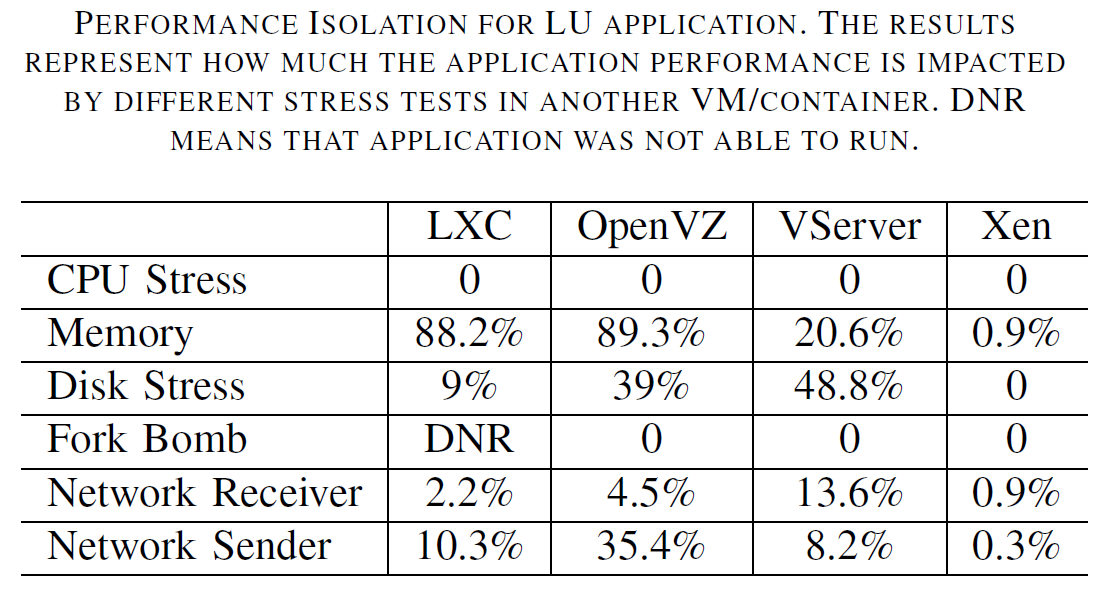
\includegraphics[width=\textwidth]{img/isolation_benchmark_suite.png}
\end{frame}